% -------------------- Packages --------------------

\documentclass{assignment}[2019/10/15]
\usepackage[lineno]{packages}[2019/11/14]

% -------------------- Settings --------------------

% Title

\title{Report for the Problem -- Flow in a Channel}
\author{Chen Xuyang}
\date{\today}
\institute{School of Mathematical Science}
\professor{Chen Suqin}
\course{Numerical Partial Differential Equations}
\subject{Numerical Partial Differential Equations}
\keywords{}

% -------------------- New commands --------------------

\newcommand{\BR}{\symbb{R}}
\newcommand{\BZ}{\symbb{Z}}
\newcommand{\diag}{\mathop{}\!\symup{diag}}
\newcommand{\pr}{\mathop{}\!\symup{Pr}}
\newcommand{\expect}{\mathop{}\!\symup{E}}
\newcommand{\cov}{\mathop{}\!\symup{Cov}}
\newcommand{\var}{\mathop{}\!\symup{Var}}

\def\multiset#1#2{\ensuremath{\left(\kern-.3em\left(\genfrac{}{}{0pt}{}{#1}{#2}\right)\kern-.3em\right)}}

\newcommand{\lr}[3]{\left#1#3\right#2}
\newcommand{\lmr}[5]{\left#1#4\middle#2#5\right#3}

\newcommand{\Oh}{\hat{\Omega}}
\newcommand{\Qh}{\hat{Q}}
\newcommand{\Linf}{L_{\infty}}
\newcommand{\ux}{{u_\xi}}
\newcommand{\ue}{{u_\eta}}
\newcommand{\uxx}{{u_{\xi\xi}}}
\newcommand{\uxe}{{u_{\xi\eta}}}
\newcommand{\uee}{{u_{\eta\eta}}}

% -------------------- Document --------------------

\begin{document}
    \maketitle
    \tableofcontents
    \clearpage

    \section{Background}

    Omitted.

    \section{Questions}

    \begin{enumerate}[1)]
        \item Introduce a mapping $T$ to transform the original domain $\Omega$ (with coordinates $x, y$) to the unit square $\hat{\Omega}$ (with coordinates $\xi, \eta$). Derive the equations and the boundary conditions in the new domain.
        \item In the transformed domain, use Taylor series expansions to derive second-order accurate finite-difference schemes for the discretization of all the derivative terms in the interior of the domain, as well as for the boundary points. You do not have to derive special schemes for the corner points, use the left boundary scheme at corner $A$, and $u = 0$ at the other three corners. Also show how to evaluate the integral in the approximate flowrate $\Qh$ numerically.
        \item Write a program, that solves the problem. Then using your program, calculate the solution and $\Qh$ using a grid size $N = 21$, for $l = 3.0, b = 0.5$ and $h = 1.0$. Compare your results with the sample solution in Figure 4 (of the problem set document).
        \item Solve the problem for $l = 3.0, h = 1.0$, and $b = 0.0, 0.5, 1.0$ (three solutions), with $N = 41$. Plot the solutions and compute $\Qh$.
        \item Calculate the convergence rate for the error in the output $\Qh$, and for the $\Linf$ and the $L_2$ norms of the solution. Do the calculation for $l = 3.0, h = 1.0$, and $b= 0.0, 0.5, 1.0$ (a total of 9 convergence plots); verify that you obtain second-order convergence. Use the grid sizes $N = 11, 21, 41, 81$. Since we don't know the exact solution, use the solution for $N = 81$ as a reference. To calculate the $\Linf$ and the $L_2$ norms, interpolate the solution obtained at the coarser meshes, to the reference mesh.
        \item Keeping $l = 3$, vary the two inputs $h = [0.1, 1.0]$ and $b = [0.0, 1.0]$. Choose points on a regular grid in this two dimensional space, with constant interval 0.1 for both $h$ and $b$ (a total of 110 combinations). Each point, an $(h, b)$ pair, represents a possible cross section. For each of these configuratioins, solve the problem (using $N = 21$) and calculate the flowrate $\hat Q$ and the moment of inertia $I$. Create a graph, using the two outputs and calculate the convex hull of these points. The convex hull. known as the Pareto optimal frontier, is a trade-off curve; for a specific choice of one output, we determine the optimal choice for the other output. Explain the results you obtain.
    \end{enumerate}

    \section{Notations}

    We will denote the upper left, lower left, lower right and upper right corner of the right-angled trapezoid by $A, C, B, D$ respectively, which is different from the original problem. And we will create the coordinate system by setting $A$ to be the original point, $AC$ to be the $x$-axis and $AD$ to be the $y$-axis, which is also different from the original problem.

    We will use $\xi_x$ to denote the partial derivative of $\xi$ by $x$, which is parametered by $\xi$ and $\eta$, instead of $x$ and $y$ ($\xi_y, \eta_x, \eta_y$ are similarly dealt with). It will be convenient for us to state the equations and boundary conditions in the new domain.

    We will use supscript to denote the value of the function $u$ and its derivatives on the point of the grid with the specific index. For example, $\uee^{i, j}$ denotes the value of second order partial derivative $\uee$ at the point $(\xi_i, \eta_j)$. This notation will not be ambiguous with the notation of power.

    \section{Transformation of the Domain and Derivation of the Problem in the New Domain}

    Let $\Oh$ denote (the interior) of the unit square, and let $T$ denote the transformation $T{:}\ (x, y)\in\overline\Omega \to (\xi, \eta)\in\overline\Oh$ where
    \begin{equation}
        \xi = \frac{x}{AC}, \quad \eta = \frac{y\cdot AC}{x\cdot BC + (AC - x)AD}.
    \end{equation}
    It is easy to verify that $T$ is a diffeomorphism which maps the boundary of $\Omega$ to the one of $\Oh$, and the vertices of $\Omega$ to the ones of $\Oh$. Denote by $A', B', C', D'$ the points $T(A), T(B), T(C), T(D)$, respectively.

    Compute the derivatives, then we have
    \begin{equation}
        \begin{aligned}
            \xi_x &= \frac{1}{AC},\\
            \xi_y &= \xi_{xx} = \xi_{yy} = 0,
        \end{aligned}
    \end{equation}
    and
    \begin{equation}
        \begin{aligned}
            \eta_x &= -\frac{(BC-AD)\eta}{AC(BC\cdot\xi + AD(1-\xi))},\\
            \eta_y &= \frac{1}{BC\cdot\xi+AD(1-\xi)},\\
            \eta_{xx} &= \frac{2(BC-AD)^2\eta}{AC^2(BC\cdot\xi+AD(1-\xi))^2},\\
            \eta_{yy} &= 0.
        \end{aligned}
    \end{equation}

    Thus in $\Oh$, we have
    \begin{equation}
        1 = -(u_{xx} + u_{yy}) = -(a\uxx+b\uxe+c\uee+d\ux+e\ue) = 1,
    \end{equation}
    where
    \begin{equation}
        \begin{aligned}
            a &= {\xi_x}^2+{\xi_y}^2 = \frac{1}{AC^2},\\
            b &= 2(\xi_x\eta_x+\xi_y\eta_y)=-\frac{2(BC-AD)\eta}{AC^2(BC\xi+AD(1-\xi))},\\
            c &= {\eta_x}^2+{\eta_y}^2,\\
            d &= \xi_{xx} + \xi_{yy} = 0,\\
            e &= \eta_{xx} + \eta_{yy} = \eta_{xx}.\\
        \end{aligned}
    \end{equation}
    The symbol $b$ is also used to denote the size of the base in the trapezoid. In the context this usage will not be ambiguous.

    On line $A'C'$, since $\eta = \text{const}$, we have
    \begin{equation}
        0=\frac{\partial u}{\partial n} = \left({\eta_x}^2+{\eta_y}^2\right)^{-1/2}\lr(){(\ux\xi_x+\ue\eta_x)\eta_x+(\ux\xi_y+\ue\eta_y)\eta_y}=c^{-1/2}\xi_x\eta_x\ue+c^{1/2}\ue.
    \end{equation}

    Similarly, on line $A'D'$ we have
    \begin{equation}
        0=\frac{\partial u}{\partial n} = \left({\xi_x}^2+{\xi_y}^2\right)^{-1/2}\lr(){(\ux\xi_x+\ue\eta_x)\xi_x+(\ux\xi_y+\ue\eta_y)\xi_y}=\xi_x\ux+\eta_x\ue.
    \end{equation}

    Consequencely, we derive the problem in the new domain
    \begin{equation}
        \begin{cases}
            -(a\uxx+b\uxe+c\uee+e\ue) = 1, &\text{in }\Oh,\\
            c^{-1/2}\xi_x\eta_x\ux+c^{1/2}\ue=0, &\text{in }A'C'\text{ and }A',\\
            \xi_x\ux+\eta_x\ue=0, &\text{in }A'D',\\
            u = 0, &\text{else}.
        \end{cases}
    \end{equation}

    \section{Discretization for the Problem and Numerical Method for Integration}

    Create a uniform grid in the closure of $\Oh$ with the constant interval $\Delta = 1/(N-1)$ with $N\times N$ points , that is to say, with the set of points
    \begin{equation}
        \left\{(\xi_i, \eta_j)\middle\vert\ \xi_i = i\Delta, \eta_j = j\Delta, 0\leq i,j\leq N-1\right\}.
    \end{equation}

    Using the method of undetermined coefficients, we can obtain the schemes of all derivative terms. We will omit this process since the conclusion is easy to verify.

    In $\Oh$, we have $1\leq i, j\leq N-2$, and
    \begin{equation}
        \begin{aligned}
            {\uxx}^{i, j} &= \frac{1}{\Delta^2}\left(u^{i+1, j}-2u^{i, j}+u^{i-1, j}\right),\\
            \uxe^{i, j} &= \frac{1}{4\Delta^2}\left(u^{i+1, j+1}+u^{i-1. j-1}-u^{i+1, j-1}-u^{i-1, j+1}\right),\\
            \uee^{i, j} &= \frac{1}{\Delta^2}\left(u^{i, j+1}-2u^{i, j}+u^{i, j-1}\right).
        \end{aligned}
    \end{equation}
    Substitute the derivative terms by the schemes in the equation $-(a\uxx+b\uxe+c\uee+e\ue) = 1$, we will derive the linear equation at $(i, j)$, which is
    \begin{equation}
        \left<\matr{A}^{i, j}, \matr{U}^{i, j}\right> = 1,
    \end{equation}
    where
    \begin{equation}
        \begin{aligned}
            \matr{A}^{i, j}&=
            \begin{bmatrix}
                -b/(4\Delta^2) & -a/\Delta^2 & b/(4\Delta^2)\\
                -c/\Delta^2+e/(2\Delta) & (2a+2c)/\Delta^2 & -c/\Delta^2-e/(2\Delta)\\
                b/(4\Delta^2) & -a/\Delta^2 & -b/(4\Delta^2)
            \end{bmatrix},\\
            \matr{U}^{i, j}&=
            \begin{bmatrix}
                u^{i-1, j-1} & u^{i-1, j} & u^{i-1, j+1}\\
                u^{i, j-1} & u^{i, j} & u^{i, j+1}\\
                u^{i+1, j-1} & u^{i+1, j} & u^{i+1, j+1}
            \end{bmatrix},
        \end{aligned}
    \end{equation}
    and the coefficients take their value at the point $(\xi_i, \eta_j)$. It will be the same in the sequel.

    In $A'D'$, we have $i = 0, 1\leq j\leq N-2$, and
    \begin{equation}
        \begin{aligned}
            \ux^{i, j} &= \frac{1}{2\Delta}\lr(){-u^{i+2, j}+4u^{i+1, j}-3u^{i, j}},\\
            \ue^{i, j} &= \frac{1}{2\Delta}\lr(){u^{i, j+1}-u^{i, j-1}}.
        \end{aligned}
    \end{equation}
    Substitute the derivative terms by the schemes in the equation $\xi_x\ux+\eta_x\ue = 0$, we will derive the linear equation at $(i, j)$, which is
    \begin{equation}
        \frac{1}{2\Delta}\lr(){-u^{i+2, j}+4u^{i+1, j}-3u^{i, j}}\xi_x+\frac{1}{2\Delta}\lr(){u^{i, j+1}-u^{i, j-1}}\eta_x = 0.
    \end{equation}

    In $A'C'$, we have $1\leq i \leq N-2, j = 0$, and
    \begin{equation}
        \begin{aligned}
            \ux^{i, j} &= \frac{1}{2\Delta}\lr(){u^{i+1, j}-u^{i-1, j}},\\
            \ue^{i, j} &= \frac{1}{2\Delta}\lr(){-u^{i, j+2}+4u^{i, j+1}-3u^{i, j}}.
        \end{aligned}
    \end{equation}
    Substitute the derivative terms by the schemes in the equation $c^{-1/2}\xi_x\eta_x\ux+c^{1/2}\ue=0$, we will derive the linear equation at $(i, j)$, which is
    \begin{equation}
        c^{-1/2}\xi_x\eta_x\frac{1}{2\Delta}\lr(){u^{i+1, j}-u^{i-1, j}}+c^{1/2}\frac{1}{2\Delta}\lr(){-u^{i, j+2}+4u^{i, j+1}-3u^{i, j}}=0
    \end{equation}

    At $A'$, we shall notice that the scheme for $\ux$ is different from the one in $A'C'$, which shall be
    \begin{equation}
        \ux^{i, j} = \frac{1}{2\Delta}\lr(){-u^{i+2, j}+4u^{i+1, j}-3u^{i, j}}.
    \end{equation}

    At other points, we have $u^{i, j} = 0$.

    Now we should organize these linear equations into a matrix form. Let $k(i, j) = iN + (j + 1)$ be a bijection, where $0\leq i, j\leq N-1, 1\leq k\leq N\times N$. Let $u^k = u^{i, j}$, and let the equation at point $(\xi_i, \eta_j)$ be the equation at row $k(i, j)$. Then we obtain a coefficient matrix $A$ of size $(N\times N, N\times N)$ and a column vector $f$ of length $N\times N$ whose elements range from 0 and 1. Solve the linear equations $\matr{A}u=f$ and rearrange the solution $u$ to its matrix form by setting $u^{i, j} = u^{k(i, j)}$, we can obtain the numerical solution of the problem.

    Finally, we shall use the composed trapezoid formula to compute the integral on $\Omega$. Recall that $T$ is the transformation map. Let $y(\xi, \eta)$ be the second component of $T^{-1}(\xi, \eta)$ and let $f$ be the function to be integrated. Then
    \begin{equation}\label{eq: ctf}
        \begin{aligned}
            \int_{\Omega}f(x, y)\symup{d}y\symup{d}x
            &= \int_0^1\int_0^{y(x, 1)}f(x, y)\symup{d}y\symup{d}x\\
            &= \sum_{i=0}^{N-1}a_i\int_0^{y(x_i, 1)}u(x_i, y)\symup{d}y\\
            &= \sum_{i=0}^{N-1}a_i\sum_{j=0}^{N-1}b_{ij}u(x_i, y_j)\\
            &= \sum_{0\leq i, j\leq N-1}a_ib_{i,j}u^{i,j},
        \end{aligned}
    \end{equation}
    where
    \begin{equation}
        a_i =
        \begin{cases}
            \Delta/2, &i = 0, N-1,\\
            \Delta, &i = 1, 2, \dotsc, N-2,
        \end{cases}
        \quad\text{and}\quad
        b_ij=
        \begin{cases}
            \Delta y(x_i, 1)/2, &j = 0, N-1,\\
            \Delta y(x_i, 1), &j = 1, 2, \dotsc, N-2.
        \end{cases}
    \end{equation}

    \section{Programs for Solving the Derived Problem in New Domain}

    The codes are placed in Appendix \ref{appx: q3}.

    Since the size of matrix \matlabinline{A} is very big, we need to use \matlabinline{sparse} function to create \matlabinline{A} to reduce the cost of memory. Since it is not recommanded by MATLAB documention to frequently modify the entries of a sparse matrix, especially to change the zero entries to non-zero values, we have create three arrays, namely \matlabinline{I}, \matlabinline{J}, \matlabinline{V} to temporarily store the non-zero entries of \matlabinline{A}. If we want to add a new entry to \matlabinline{A}, then we append the row to \matlabinline{I}, append the column to \matlabinline{J} and append the value to \matlabinline{V}. After every entry is stored, we use the command \matlabinline{A = sparse(I, J, V)} to construct the sparse matrix \matlabinline{A}.

    Also, we have created custom functions to change between 2-D indexs and 1-D indexs, where errors will be thrown if the inputs are out of range. It helps us to locate bugs and it is a common mistake that the size of \matlabinline{A} goes wrong.

    To plot the contour lines, we need to carefully tranform the coordinate systems to the one in the original problem. Need to take care of the output of the \matlabinline{meshgrid} function. Sometimes we need to take composite of the two output matrixs to match our solution matrix.

    We have a pretty good result with our codes. Our figures \ref{fig: q3} are very similar to the sample and our numerical value of the flowrate is slightly bigger than the sample, which is 0.059467. It may be caused by the error from composed trapezoid formula.

    \begin{figure}[htb]
        \begin{subfigure}[b]{0.49\textwidth}
            \centering
            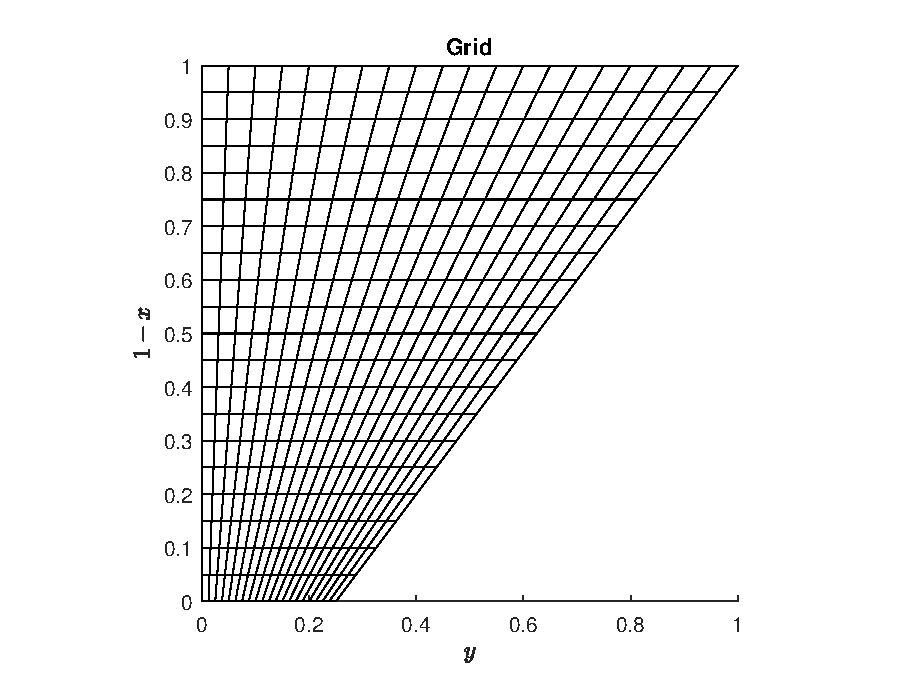
\includegraphics[width=7cm]{3-grid.eps}
            \caption{Discretization Grid in the Original Domain.}
        \end{subfigure}
        \hfill
        \begin{subfigure}[b]{0.49\textwidth}
            \centering
            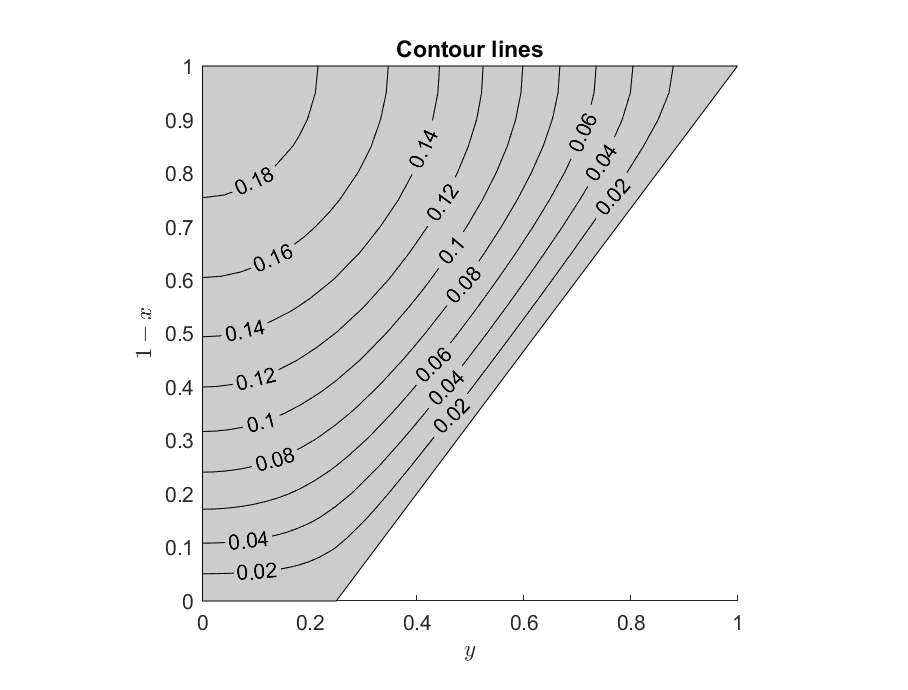
\includegraphics[width=7cm]{3-contour.eps}
            \caption{Contour Lines in the Original Domain.}
        \end{subfigure}
        \caption{Discretization Grid and Contour Lines of the Solutions for $N = 21, l = 3.0, b = 0.5, h = 1.0$.}
        \label{fig: q3}
    \end{figure}

    \section{More Solutions and More Flowrates}

    The codes are placed in Appendix \ref{appx: q4}.

    Fortunately, our programs perform perfectly at the case that $b = 0.0$ so we do not need to do any modifications to the previous codes. Refer \ref{fig: q4} for the figure. The numerical value of the flowrate is 0.046582, 0.059597, 0.028569 for $N = 41$ and $b = 0.0, 0.5, 1.0$ respectively.

    \begin{figure}[htb]
        \begin{subfigure}[b]{0.32\textwidth}
            \centering
            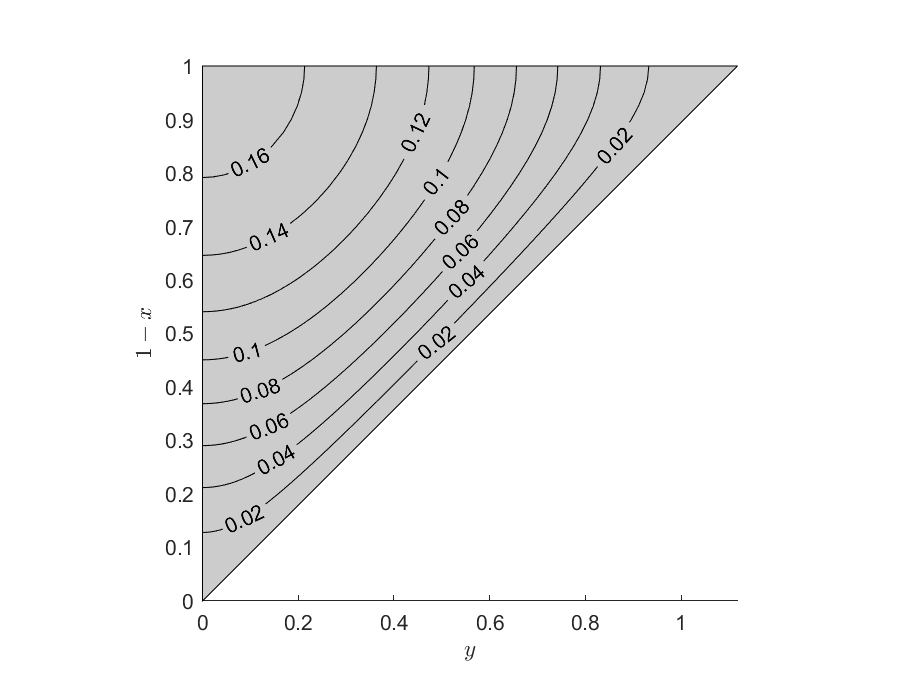
\includegraphics[width=5cm]{4-contour-1.eps}
            \caption{$b = 0.0$.}
        \end{subfigure}
        \hfill
        \begin{subfigure}[b]{0.32\textwidth}
            \centering
            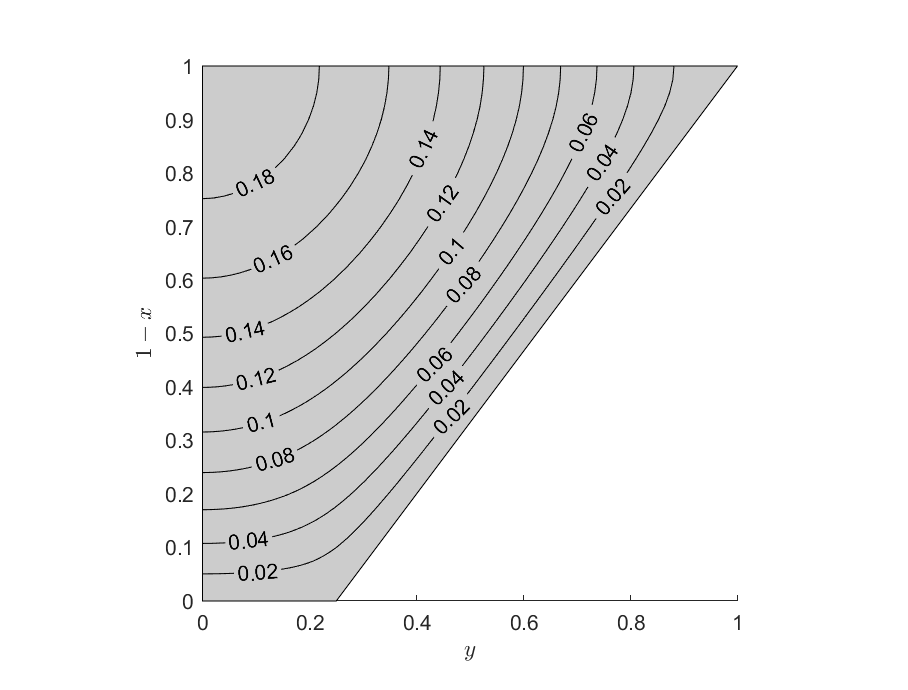
\includegraphics[width=5cm]{4-contour-2.eps}
            \caption{$b = 0.5$.}
        \end{subfigure}
        \hfill
        \begin{subfigure}[b]{0.32\textwidth}
            \centering
            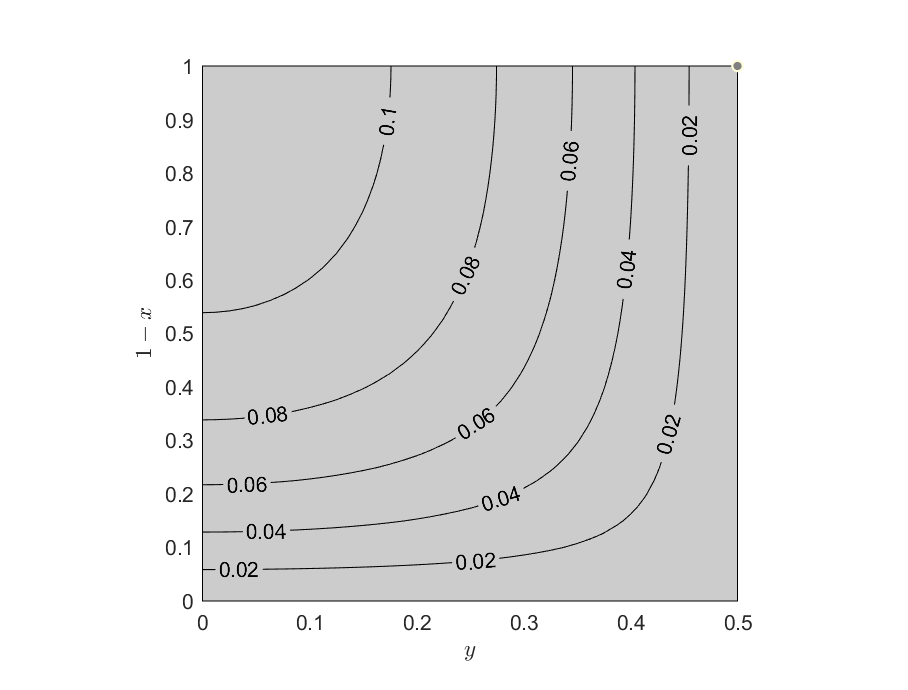
\includegraphics[width=5cm]{4-contour-3.eps}
            \caption{$b = 1.0$.}
        \end{subfigure}
        \caption{Contour Lines of the Solutions for $N = 21, l = 3.0, h = 1.0$ and Different Values of $b$.}
        \label{fig: q4}
    \end{figure}

    \section{Convergence Rate for the Error of the Flowrate and the Norms of the Solution}

    The codes are placed in Appendix \ref{appx: q5}.

    To get the linear fitting of the data points, we have manually constructed the corresponding linear equations where the number of equations is larger than the number of variables. Then we have used \matlabinline{\\} to obtain the least square solution, where the positive part of the slope is the convergence rate we needed.

    Similar to the modified $L_2$ norm in the 1-D case, we have defined a {\it weighted} $L_2$ norm of our matrix related to the grid of the right-angled trapezoid, that is the numerical value of the integral $\int (\Delta u)^2$ calculated by composed trapezoid formula developed in \ref{eq: ctf}.

    From the figures \ref{fig: q5-Q}, \ref{fig: q5-Linf} and \ref{fig: q5-L2} we can see that we obtain second-order convergence for $\hat Q$ and $L_2$ norm, but not $L_\infty$ norm with $b = 0.0, 0.5$. Sincerely I don't know the reason of it.

    \begin{figure}[htb]
        \begin{subfigure}[b]{0.32\textwidth}
            \centering
            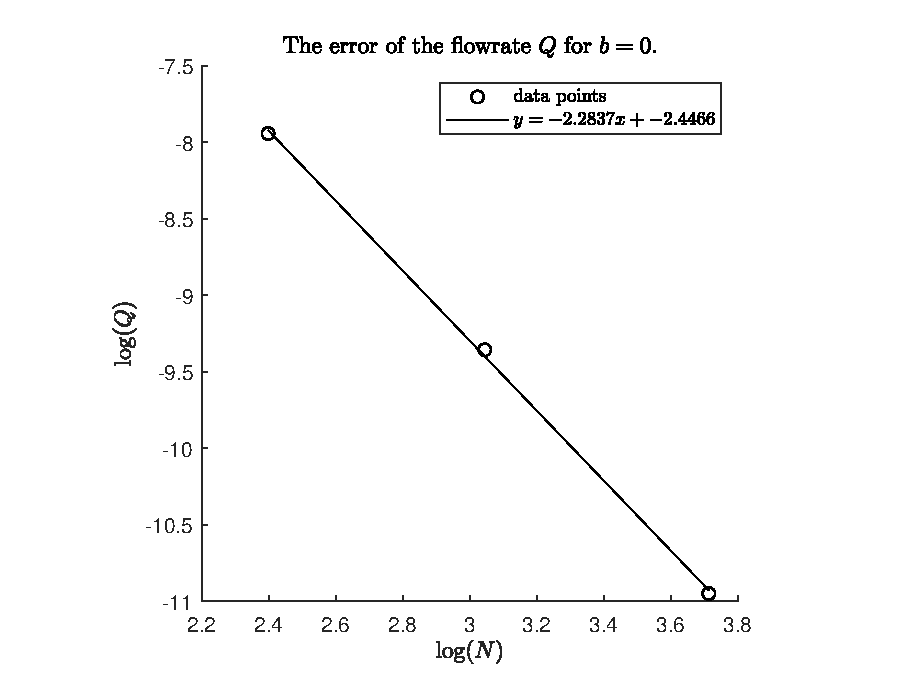
\includegraphics[width=5cm]{5-Q-1.eps}
            \caption{$b = 0.0, \text{scope} = -2.2837$.}
        \end{subfigure}
        \hfill
        \begin{subfigure}[b]{0.32\textwidth}
            \centering
            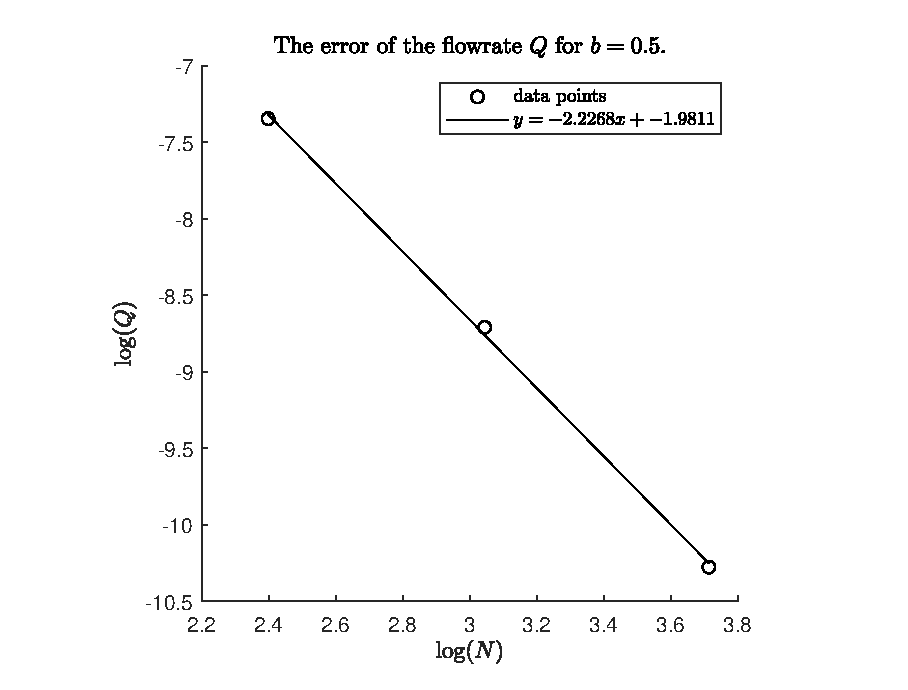
\includegraphics[width=5cm]{5-Q-2.eps}
            \caption{$b = 0.5, \text{scope} = -2.2268$.}
        \end{subfigure}
        \hfill
        \begin{subfigure}[b]{0.32\textwidth}
            \centering
            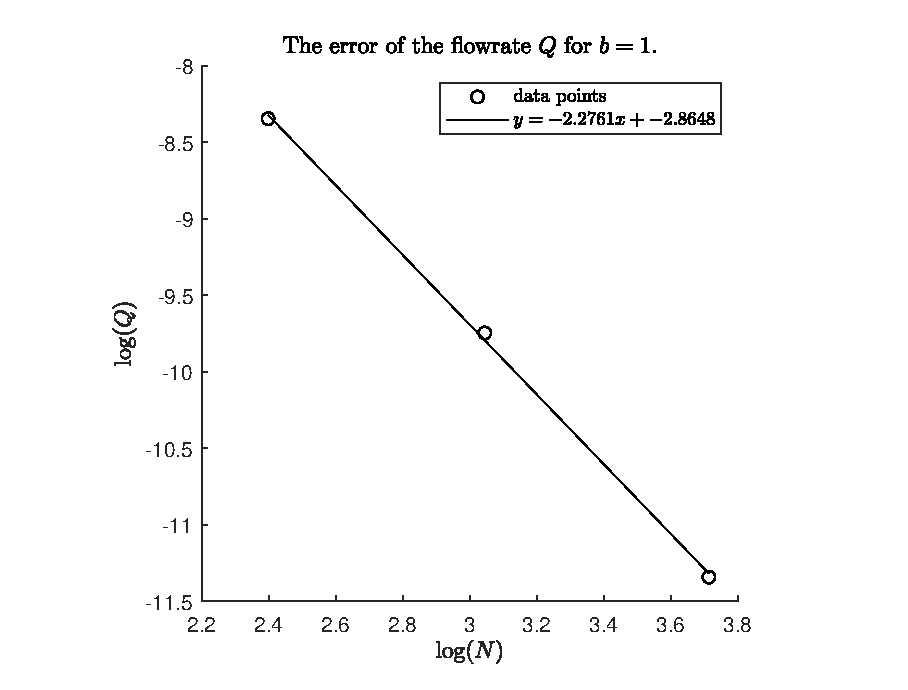
\includegraphics[width=5cm]{5-Q-3.eps}
            \caption{$b = 1.0, \text{scope} = -2.2761$.}
        \end{subfigure}
        \caption{Convergence plots for the error of the flowrate $\hat Q$ for $l = 3.0, h = 1.0$ and different values of $b$ where the $x$-axis represents $\log N$ and the $y$-axis represents $\log \Delta \hat{Q}$.}
        \label{fig: q5-Q}
    \end{figure}

    \begin{figure}[htb]
        \begin{subfigure}[b]{0.32\textwidth}
            \centering
            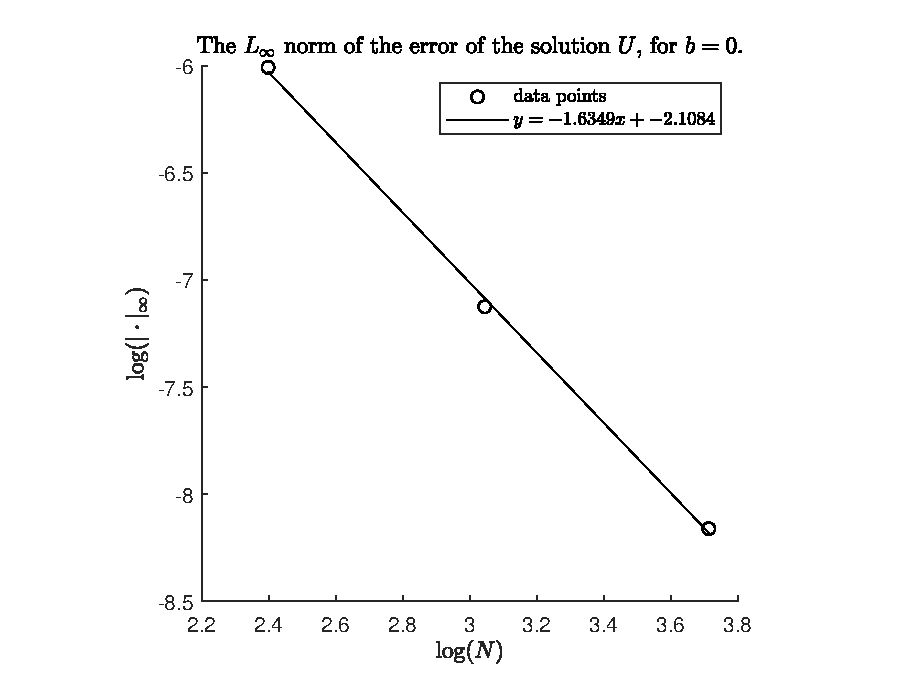
\includegraphics[width=5cm]{5-Linf-1.eps}
            \caption{$b = 0.0, \text{scope} = -1.6349$.}
        \end{subfigure}
        \hfill
        \begin{subfigure}[b]{0.32\textwidth}
            \centering
            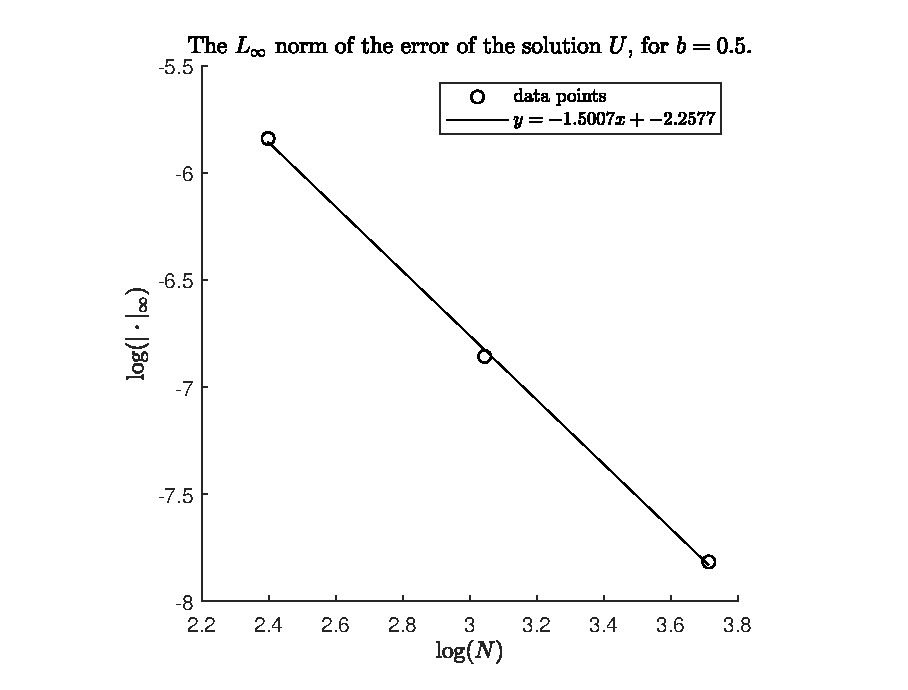
\includegraphics[width=5cm]{5-Linf-2.eps}
            \caption{$b = 0.5, \text{scope} = -1.5007$.}
        \end{subfigure}
        \hfill
        \begin{subfigure}[b]{0.32\textwidth}
            \centering
            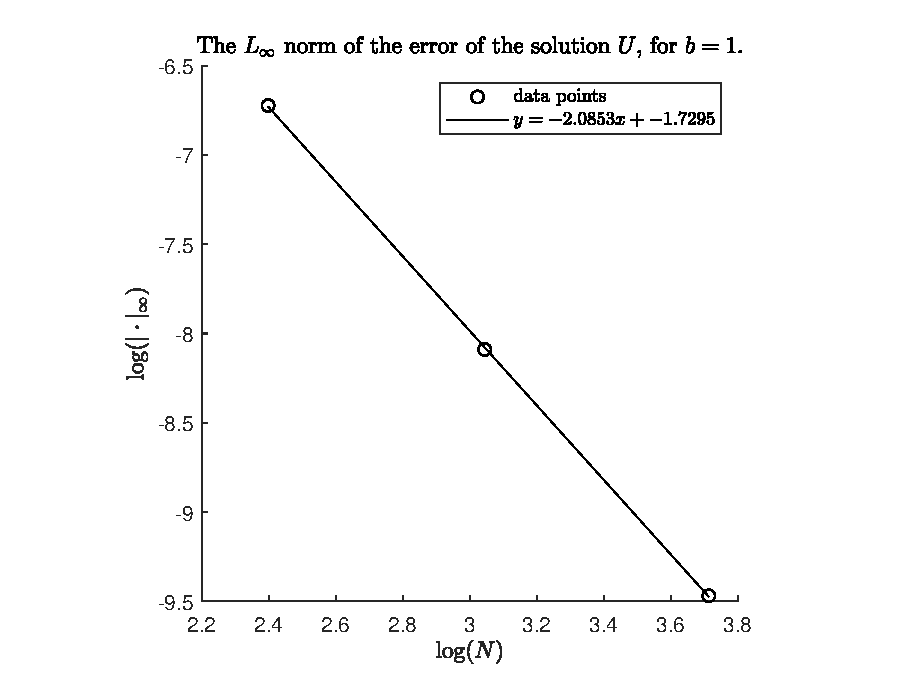
\includegraphics[width=5cm]{5-Linf-3.eps}
            \caption{$b = 1.0, \text{scope} = -2.0853$.}
        \end{subfigure}
        \caption{Convergence plots for the $L_\infty$ norms of the solution $u$ for $l = 3.0, h = 1.0$ and different values of $b$ where the $x$-axis represents $\log N$ and the $y$-axis represents $\log  \norm{\Delta u}_\infty$.}
        \label{fig: q5-Linf}
    \end{figure}

    \begin{figure}[htb]
        \begin{subfigure}[b]{0.32\textwidth}
            \centering
            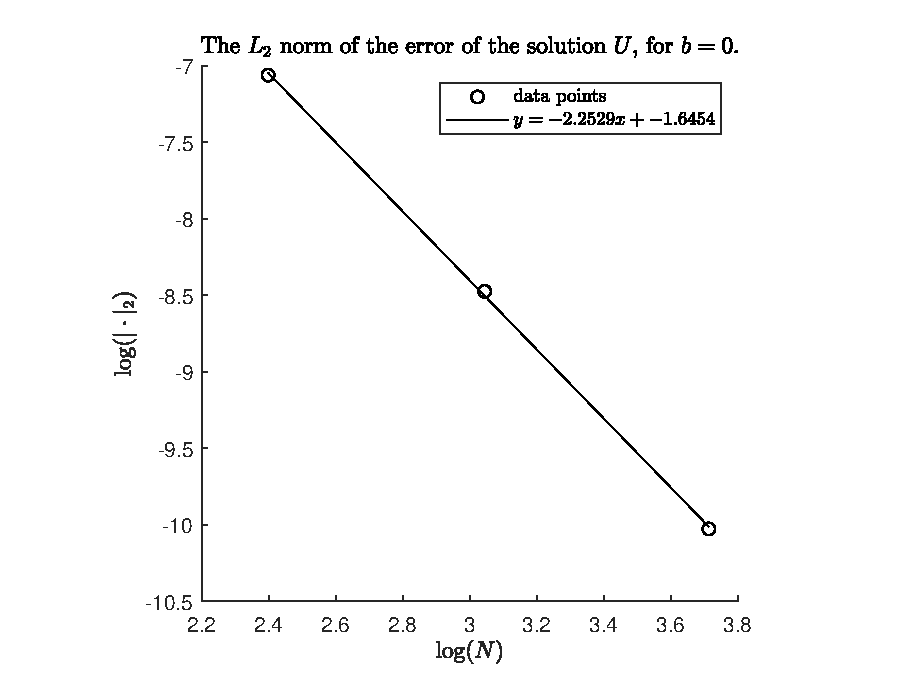
\includegraphics[width=5cm]{5-L2-1.eps}
            \caption{$b = 0.0, \text{scope} = -2.2529$.}
        \end{subfigure}
        \hfill
        \begin{subfigure}[b]{0.32\textwidth}
            \centering
            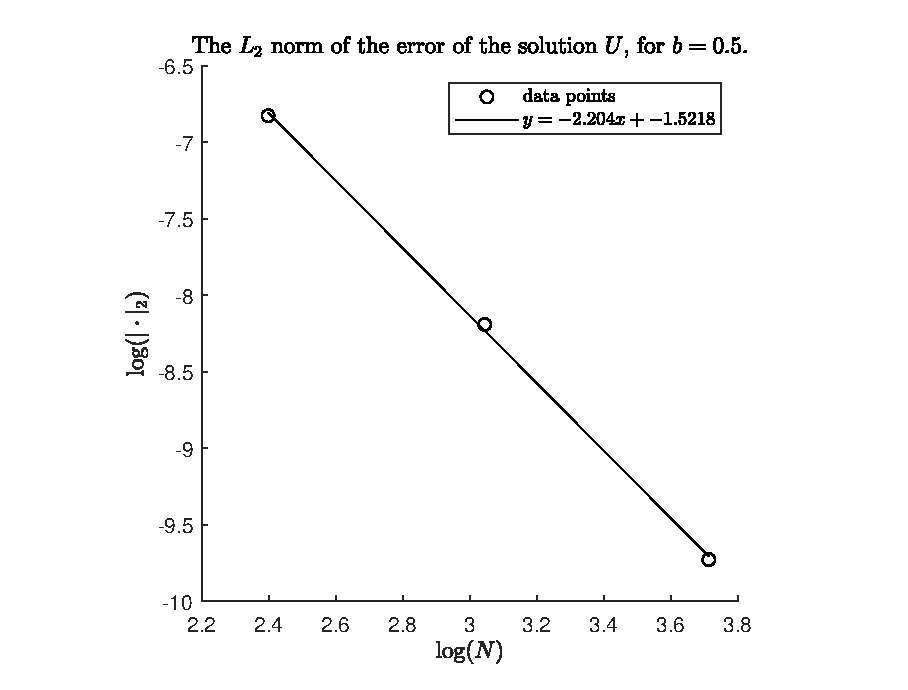
\includegraphics[width=5cm]{5-L2-2.eps}
            \caption{$b = 0.5, \text{scope} = -2.2040$.}
        \end{subfigure}
        \hfill
        \begin{subfigure}[b]{0.32\textwidth}
            \centering
            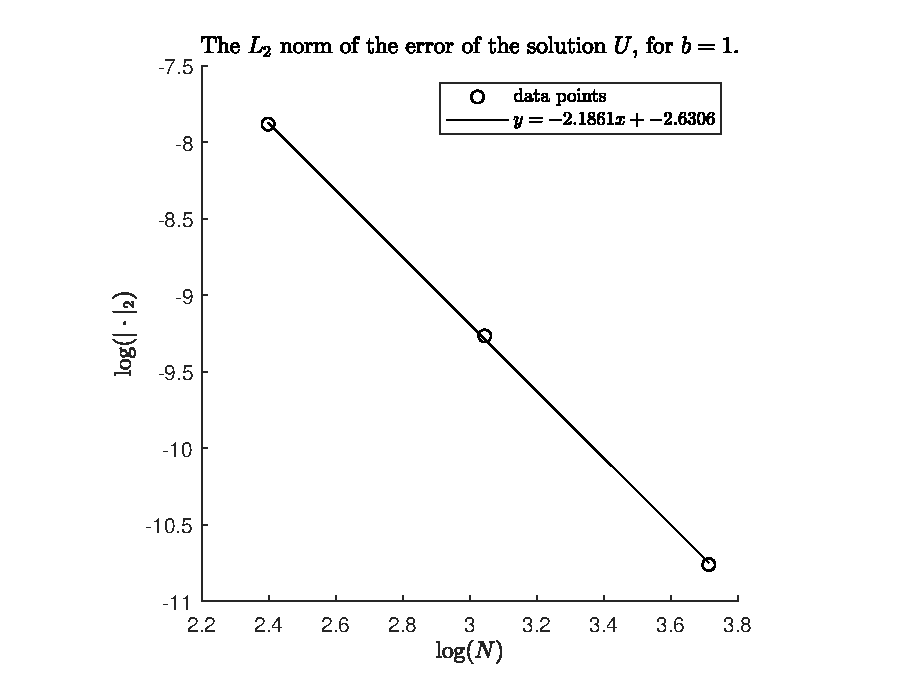
\includegraphics[width=5cm]{5-L2-3.eps}
            \caption{$b = 1.0, \text{scope} = -2.1861$.}
        \end{subfigure}
        \caption{Convergence plots For the $L_1$ norms of the solution $u$ for $l = 3.0, h = 1.0$ and different values of $b$ where the $x$-axis represents $\log N$ and the $y$-axis represents $\log \Delta \norm{\Delta u}_1$.}
        \label{fig: q5-L2}
    \end{figure}

    \section{Pareto Optimal Frontier}

    The codes are placed in Appendix \ref{appx: q6}.

    The convex hull in the figure \ref{fig: q6} is called the Pareto optimal frontier, which is a trade-off curve. If we fix the moment of inertia $I$, then the maxium and minimum possible flowrate $\hat Q$ is placed on the convex hull. Hence the frontier can help us make decisions.

    \begin{figure}[htb]
        \centering
        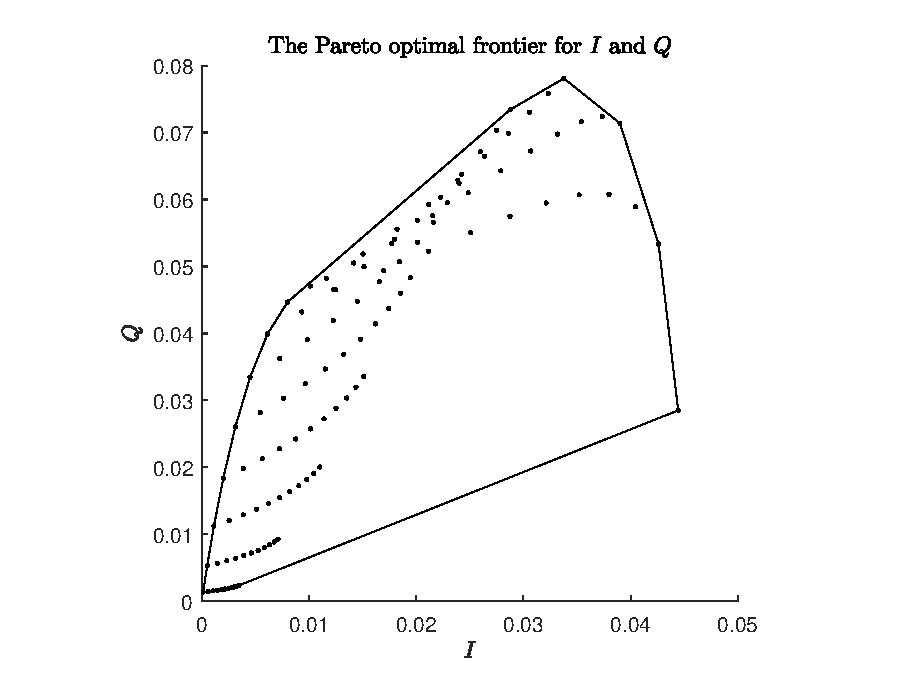
\includegraphics[width=7cm]{6-curve.eps}
        \caption{The Pareto optimal frontier for the moment of inertia $I$ and the flowrate $\hat Q$.}
        \label{fig: q6}
    \end{figure}

    \clearpage\appendix

    \section{Codes for Solving the Problem in New Domain}\label{appx: q3}

    \matlabinputlisting[caption={Main Script for Question 3}]{question_3.m}
    \matlabinputlisting[caption={Function for Solving the Problem with Given Parameters}]{solve_problem.m}
    \matlabinputlisting[caption={Function for Plotting the Discretization Grid in Original Domain}]{plot_grid.m}
    \matlabinputlisting[caption={Function for Plotting the Contour Lines of a Given Solution}]{plot_contour.m}
    \matlabinputlisting[caption={Function for Computing Numerical Integral in the Original Domain by Composed Trapezoid Formula}]{compute_flowrate.m}
    \matlabinputlisting[caption={Function for Getting More Constants From Given Parameters to Simplify the Codes}]{get_constants.m}

    \section{Codes for Computing More Solutions and More Flowrates}\label{appx: q4}

    \matlabinputlisting[caption={Main Script for Question 4}]{question_4.m}

    \section{Codes for Computing the Convergence Rate for the Error of the Flowrate and the Norms of the Solution}\label{appx: q5}

    \matlabinputlisting[caption={Main Script for Question 5}]{question_5.m}

    \section{Codes for Plotting the Pareto Optimal Frontier}\label{appx: q6}

    \matlabinputlisting[caption={Main Script for Question 6}]{question_6.m}
\end{document}
